% Metódy inžinierskej práce

\documentclass[10pt,twocolumn,twoside,slovak,a4paper]{article}

\usepackage[slovak]{babel}
%\usepackage[T1]{fontenc}
\usepackage[IL2]{fontenc} % lepšia sadzba písmena Ľ než v T1
\usepackage[utf8]{inputenc}
\usepackage{graphicx}
\usepackage{url} % príkaz \url na formátovanie URL
\usepackage{hyperref} % odkazy v texte budú aktívne (pri niektorých triedach dokumentov spôsobuje posun textu)
\usepackage{transparent}
\usepackage{amsmath}
\usepackage{eso-pic}
\usepackage{graphicx}
\graphicspath{ {./images/} }

\usepackage{cite}
%\usepackage{times}

\pagestyle{headings}

\title{Ako môže pomôcť detekcia emócii v odporúčacích systémoch\thanks{Semestrálny projekt v predmete Metódy inžinierskej práce, ak. rok 2024/25, vedenie: Pavol Baťalík}} % meno a priezvisko vyučujúceho na cvičeniach

\author{Richard Klein\\[2pt]
	{\small Slovenská technická univerzita v Bratislave}\\
	{\small Fakulta informatiky a informačných technológií}\\
	{\small \texttt{xklein@stuba.sk}}
	}

\date{\small 30. september 2024} % upravte



\begin{document}

\maketitle

\begin{abstract}
\AddToShipoutPicture*{
    \put(0,0){
        \parbox[b][\paperheight]{\paperwidth}{%
            \vfill
            \centering
            {\transparent{0.8}
\includegraphics[width=0.5\textwidth]{STU-FIIT-nvf}}%
            \vfill
        }
    }
}
Emócie sú pre ľudí kľúčové, pretože ovplyvňujú nielen to, ako vnímame svet okolo seba, ale aj to, ako reagujeme na rôzne podnety. Schopnosť rozpoznávať a prejavovať emócie nám umožňuje vytvárať nové medziľudské vzťahy, reagovať na rôzne situácie empaticky a rozhodovať sa na základe nielen faktov, ale aj emocionálnych faktorov. Jedna z ďalších dôležitých veci je pre väčšinu z nás aj náš osobný počítač, ktorý nám pomáha našu prácu a rozhodovanie urýchľovať. Počítač dokáže o nás získať množstvo informácií, od našich záujmov a nedávnych nákupov až po históriu vyhľadávania a trávenie času na sociálnych sieťach. Vie, čo robíme, kedy a kde to robíme. Napriek tomu, ako dobre nás počítače poznajú z hľadiska našich denných zvykov, stále nedokážu presne rozpoznať, ako sa cítime. Nevie nám žiadnym spôsobom zlepšiť náladu. Ale čo ak by vedela vyčítať emócie používateľa a na základe toho sa snažil pomôcť? Tento článok sa zaoberá porovnaním metód, akými môže váš počítač zistiť ako sa práve cítite a následne jeho implementáciu do odporúčacieho systému v zábavnom priemysle, hlavne pre online streamovacie platformy ako je napríklad Netflix pre filmy a seriály alebo platforma Spotify pre hudbu a podcasty. Medzi spomínané metódy bude patriť čítanie emócií len pomocou používania vstupných zariadený, čiže počítačovú myš a klávesnicu alebo pomocou kamery základe tvárových svalov. 
\end{abstract}



\section{Úvod}
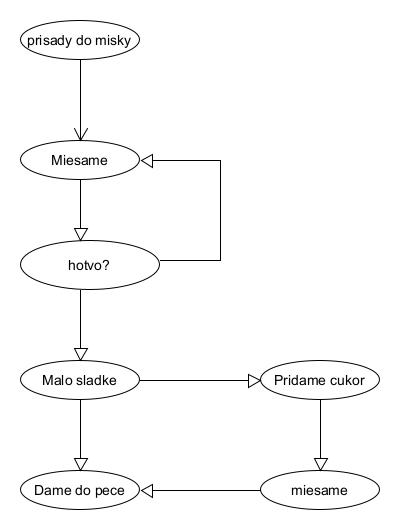
\includegraphics[width=\textwidth,height=15cm]{Recept_diagram}
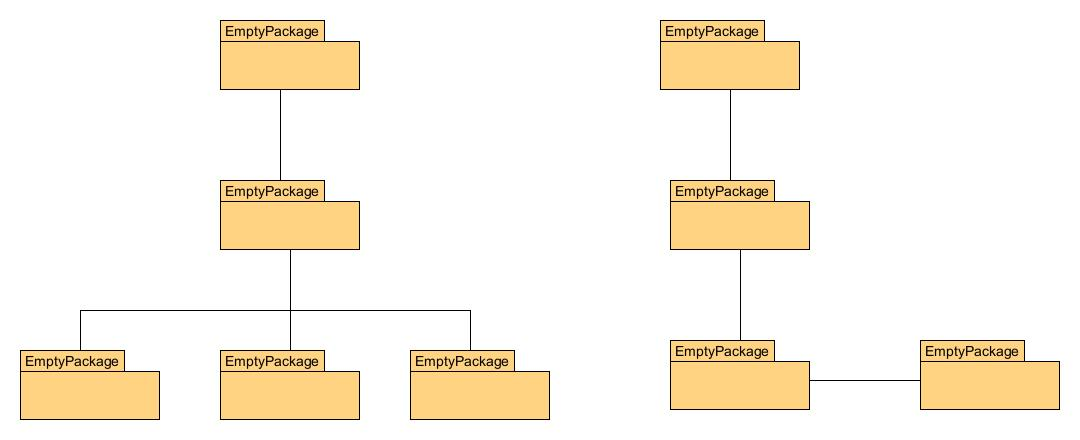
\includegraphics[width=\textwidth]{Infrastruktura_diagram}

\[ \left( \begin{array}{cc}
1 & 0 \\
0 & 1
\end{array} \right)








\end{document}
